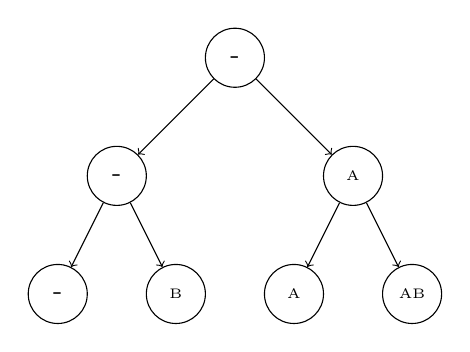
\begin{tikzpicture}[every node/.style={draw,circle, minimum size=0.75cm}, scale=0.75]
	\node at (3, 4) (R) 	{-};
	\node at (5, 2) (RA)	{\tiny A};
	\node at (1, 2) (RO)	{-};
	\node at (6, 0) (RAB)	{\tiny AB};
	\node at (4, 0) (RAO)	{\tiny A};
	\node at (2, 0) (ROB)	{\tiny B};
	\node at (0, 0) (ROO)	{-};

	\draw [->] (R) edge (RA) (R) edge (RO);
	\draw [->] (RA) edge (RAO) (RA) edge (RAB);
	\draw [->] (RO) edge (ROO) (RO) edge (ROB);
\end{tikzpicture}